\section{Experiments}
\label{sec:expt}

\begin{table*}[t]
\centering
\small
\renewcommand{\arraystretch}{1.3}
\caption{\textbf{Main results on the LongBench benchmark.} We compare DeltaKV against state-of-the-art baselines across varying model scales. \textbf{KR} and \textbf{CR} denote the KV Cache Keep Ratio and Compute Ratio, respectively. Detailed calculation methods are provided in Appendix~\ref{app:sect:kr_cr}. DeltaKV marked with $^{\dagger}$ indicates the variant utilizing a lightweight decompressor for enhanced inference efficiency. ``4-bit'' indicates that we further quantize only the compressed KV Cache to further reduce GPU memory consumption.}
\label{tab:longbench_perf}
\resizebox{0.99\linewidth}{!}{
\begin{tabular}{lcc ccccccc}
\toprule
\textbf{Method}  & \textbf{KR $\downarrow$} & \textbf{CR $\downarrow$}&
\textbf{Single-Doc $\uparrow$} &
\textbf{Multi-Doc $\uparrow$} &
\textbf{Summ. $\uparrow$} &
\textbf{Few-Shot $\uparrow$} &
\textbf{Synthetic $\uparrow$} &
\textbf{Code $\uparrow$} &
\textbf{Overall $\uparrow$} \\
\midrule
\rowcolor[HTML]{E7F3FF} 
\textit{Llama-3.1-8B}~\cite{grattafiori2024llama3}       & 100&100& 45.3 & 46.2 & 28.7 & 69.4 & 52.7 & 57.9 & 50.0 \\
% \midrule
\textbf{SnapKV}~\cite{li2024snapkv}                   & 30&30& \underline{44.5} & 46.4 & 26.5 & 68.2 & 52.7 & \underline{60.3} & 49.8 \\
\textbf{PyramidKV}~\cite{cai2024pyramidkv}                  & 30&30& 44.1 & 46.3 & 26.0 & 68.5 & 52.6 & 59.1 & 49.5 \\
\textbf{AdaKV}~\cite{feng2025adakv}                       & 30&30& 44.7 & 46.5 & 26.6 & 69.3 & 52.7 & 58.3 & 49.7 \\
% \textbf{KIVI}~\cite{liu2024kivi}                        & 25&100& 44.8 & 46.2 & 29.0 & 69.5 & 53.8 & 59.8 & 50.5 \\
\textbf{Quest}~\cite{tang2024quest}                       & 100&30& 44.4 & 46.2 & \textbf{29.3} & 69.0 & 53.1 & 57.6 & 50.0 \\
\textbf{OmniKV}~\cite{hao2025omnikv}                      & 100&30& \textbf{44.8} & 46.1 & \underline{28.9} & 68.9 & 52.8 & 59.9 & 50.2 \\
\quad \textbf{+DeltaKV}$^\dagger$  & 45&30& 43.2 & \textbf{46.8} & 27.7 & 69.5 & \textbf{54.8} & 59.7 &\underline{50.3}\\
\quad \textbf{+DeltaKV}            & 45&30& 44.4 & 45.9 & 27.6 & \underline{69.7} & 53.4 & 60.2 & 50.2 \\
\quad \quad \textbf{+4-bit}              & 29&30& 43.3 & \underline{46.6} & 27.3 & \textbf{69.8} & \underline{54.4} & \textbf{60.5} &\textbf{50.3}\\
\midrule
% 20% 比例
\textbf{SnapKV}~\cite{li2024snapkv}                       & 20&20& \underline{42.9} & 45.4 & 25.8 & \underline{68.8} & \underline{54.8} & 57.4 & 49.2 \\
\textbf{Quest}~\cite{tang2024quest}                       & 100&20& 42.2 & \textbf{46.9} & \textbf{28.8} & \textbf{68.9} & 54.9 & 56.5 & 49.7 \\
\textbf{OmniKV}~\cite{hao2025omnikv}                      & 100&20& \textbf{43.0} & 45.7 & \underline{27.5} & 68.6 & \textbf{54.9} & \textbf{60.8} & \textbf{50.1} \\
\quad \textbf{+DeltaKV}$^\dagger$  & 43 & 20 & 42.7 & \underline{46.2} & 26.2 & 68.7 & 54.3 & \underline{60.5} & \underline{49.8}\\
\midrule
\rowcolor[HTML]{D9EAD3} 
\textit{Qwen2.5-7B}~\cite{yang2025qwen2_1m}         & 100&100& 42.5 & 49.6 & 28.6 & 68.7 & 53.8 & 42.5 & 47.6 \\
% \midrule
\textbf{SnapKV}~\cite{li2024snapkv}                      & 30&30& 41.7 & 48.8 & 26.6 & 68.3 & \textbf{54.5} & \textbf{41.8} & 47.0 \\
\textbf{PyramidKV}~\cite{cai2024pyramidkv}                   & 30&30& 40.6 & 48.7 & 24.4 & 67.7 & \underline{54.5} & 40.6 & 46.1 \\
\textbf{Palu}~\cite{chang2025palu}                      & 50&100& 34.4 & 35.6 & 27.5 & 68.7 & 45.0 & 21.3 & 38.8 \\
\textbf{OmniKV}~\cite{hao2025omnikv}                      & 100&30& \textbf{41.9} & \textbf{49.4} & \textbf{28.4} & \underline{69.1} & 54.0 & 41.5 & \textbf{47.4} \\
\quad \textbf{+DeltaKV}            & 48&30& \underline{41.8} & \underline{49.0} & \underline{27.7} & \textbf{69.1} & 53.3 & \underline{41.7} & \underline{47.1} \\
\midrule
\rowcolor[HTML]{FFF2CC}
\textit{Qwen2.5-32B}~\cite{team2024qwen2}        & 100&100& 42.7 & 54.3 & 27.3 & 67.6 & 56.0 & 42.6 & 48.4 \\
% \midrule
\textbf{SnapKV}~\cite{li2024snapkv}                      & 20&20& 39.5& 53.8& 24.6& \underline{67.2}& \underline{56.0}& 41.7& 47.1\\
\textbf{OmniKV}~\cite{hao2025omnikv} &  100&20& \textbf{42.4}& \underline{54.2}& \textbf{26.9}& \textbf{67.2}& \textbf{56.1}& \underline{41.7}& \textbf{48.1}\\
\quad \textbf{+DeltaKV}& 44&20& \underline{41.9} & \textbf{54.2}& \underline{26.2} & 66.1& 55.4& \textbf{42.1}& \underline{47.7}\\
\bottomrule
\end{tabular}
}
\end{table*}
\setlength{\textfloatsep}{1.5em}


% \begin{table*}[t]
% \centering
% \small
% \caption{LongBench category-wise averages and overall average.}
% \label{tab:longbench_perf}
% % \resizebox{0.99\linewidth}{!}{
% \begin{tabular}{lcc ccccccc}
% \toprule
% \textbf{Method}  & \textbf{KR} & \textbf{CR}&
% \textbf{Single-Doc} &
% \textbf{Multi-Doc} &
% \textbf{Summ.} &
% \textbf{Few-Shot} &
% \textbf{Synthetic} &
% \textbf{Code} &
% \textbf{Overall} \\
% \midrule
% \rowcolor[HTML]{E7F3FF} 
% \textit{Llama-3.1-8B}       & 100&100& 45.3 & 46.2 & 28.7 & 69.4 & 52.7 & 57.9 & 50.0 \\
% % \midrule
% SnapKV~\textcolor{gray}{\scriptsize (NeurIPS'24)}                   & 30&30& 44.5 & 46.4 & 26.5 & 68.2 & 52.7 & 60.3 & 49.8 \\
% PyramidKV~\textcolor{gray}{\scriptsize (COLM'25)}                  & 30&30& 44.1 & 46.3 & 26.0 & 68.5 & 52.6 & 59.1 & 49.5 \\
% AdaKV~\textcolor{gray}{\scriptsize (NeurIPS'25)}                       & 30&30& 44.7 & 46.5 & 26.6 & 69.3 & 52.7 & 58.3 & 49.7 \\
% KIVI~\textcolor{gray}{\scriptsize (ICML'24)}                        & 25&100& 44.8 & 46.2 & 29.0 & 69.5 & 53.8 & 59.8 & 50.5 \\
% Quest~\textcolor{gray}{\scriptsize (ICML'24)}                       & 100&30& 44.4 & 46.2 & 29.3 & 69.0 & 53.1 & 57.6 & 50.0 \\
% OmniKV~\textcolor{gray}{\scriptsize (ICLR'25)}                      & 100&30& 44.8 & 46.1 & 28.9 & 68.9 & 52.8 & 59.9 & 50.2 \\
% \quad +\textbf{DeltaKV}            & 45&30& 44.4 & 45.9 & 27.6 & 69.7 & 53.4 & 60.2 & 50.2 \\
% \quad \quad +KIVI-4-bit              & 29&30& 43.3 & 46.6 & 27.3 & 69.8 & 54.4 & 60.5 &50.3\\
% \quad +\textbf{DeltaKV}$^\dagger$  & 45&30& 43.2 & 46.8 & 27.7 & 69.5 & 54.8 & 59.7 &50.3\\
% \midrule
% \rowcolor[HTML]{D9EAD3} 
% \textit{Qwen2.5-7B}         & 100&100& 42.5 & 49.6 & 28.6 & 68.7 & 53.8 & 42.5 & 47.6 \\
% % \midrule
% SnapKV                      & 30&30& 41.7 & 48.8 & 26.6 & 68.3 & 54.5 & 41.8 & 47.0 \\
% PyramidKV                   & 30&30& 40.6 & 48.7 & 24.4 & 67.7 & 54.5 & 40.6 & 46.1 \\
% Palu~\textcolor{gray}{\scriptsize (ICLR'25)}                        & 50&100& 34.4 & 35.6 & 27.5 & 68.7 & 45.0 & 21.3 & 38.8 \\
% OmniKV                      & 100&30& 41.9 & 49.4 & 28.4 & 69.1 & 54.0 & 41.5 & 47.4 \\
% \quad +\textbf{DeltaKV}            & 48&30& 41.8 & 49.0 & 27.7 & 69.1 & 53.3 & 41.7 & 47.1 \\
% \midrule
% \rowcolor[HTML]{FFF2CC}
% \textit{Qwen2.5-32B}        & 100&100& 42.7 & 54.3 & 27.3 & 67.6 & 56.0 & 42.6 & 48.4 \\
% % \midrule
% SnapKV                      & 20&20& 39.5& 53.8& 24.6& 67.2& 56.0& 41.7& 47.1\\
% OmniKV& 100&20& 42.4& 54.2& 26.9& 67.2& 56.1& 41.7& 48.1\\
% \quad +\textbf{DeltaKV}& 44&20& 41.9& 54.2& 26.2& 66.1& 55.4& 42.1& 47.7\\
% \bottomrule
% \end{tabular}
% % }
% \end{table*}

\subsection{Experimental Setup}
\label{sec:expt:setup}

\paragraph{Training Configuration}
We evaluate DeltaKV on \textbf{Llama3.1-8B-Instruct}~\cite{grattafiori2024llama3}, \textbf{Qwen2.5-7B-Instruct-1M}~\cite{yang2025qwen2_1m}, \textbf{Qwen2.5-32B-Instruct}~\cite{team2024qwen2}, and \textbf{DeepSeek-R1-Distill-Qwen-7B}~\cite{guo2025deepseekr1}. 
%%%
DeltaKV is lightweight to train, requiring only \textbf{160M tokens} and can be fully trained in \textbf{8 GPU hours} for standard 7B/8B models on a single NVIDIA RTX PRO 6000.
%%%
Full hyperparameters, hardware details, and training overhead are provided in Appendix~\ref{subsec:detailed_settings}.

\paragraph{Baselines}
We compare against three categories of strong baselines:
%%%
(1) \textit{Static eviction} methods (\textbf{SnapKV}~\cite{li2024snapkv}, \textbf{PyramidKV}~\cite{cai2024pyramidkv}, and \textbf{AdaKV}~\cite{feng2025adakv}), which permanently remove tokens identified as unimportant and may lose critical information in multi-turn dialogues or complex reasoning scenarios. 
%%%
(2) \textit{Dynamic sparsity} methods (\textbf{Quest}~\cite{tang2024quest} and \textbf{OmniKV}~\cite{hao2025omnikv}), which select tokens adaptively for sparse attention during computation but retain the full KV Cache. 
%%%
(3) \textit{KV cache compression}, where \textbf{Palu}~\cite{chang2025palu} is most related but only considers individual token information and ignores inter-token similarity. 

\paragraph{Evaluation}
To comprehensively evaluate DeltaKV, we conduct experiments on \textbf{LongBench}~\cite{bai2024longbench} (general long-context understanding), \textbf{SCBench}~\cite{li2024scbench} (multi-turn dialogue), and \textbf{AIME}~\cite{maa_aime} (complex reasoning). 
%%%
To quantify the efficiency gains in terms of memory and computation, we report the KV Cache Keep Ratio (\textbf{KR}) and KV Cache Compute Ratio (\textbf{CR}). 
Dataset details and metric definitions are provided in Appendix~\ref{app:sect:eval_details}.
\vspace{-0.25em}

\subsection{Downstream Performance}
\label{sec:expt:performance}

\vspace{-0.25em}
\paragraph{Simple Single-step LongBench} 
Table~\ref{tab:longbench_perf} shows that DeltaKV achieves competitive performance across various models and scales on LongBench, matching the results of OmniKV. 
%%%
Furthermore, compared to OmniKV, DeltaKV is more memory-efficient, typically reducing KR by about half. It can also be combined with KV quantization for further memory savings without noticeable performance loss.

\paragraph{Complex Multi-turn SCBench} 
Results in Table~\ref{tab:scbench_perf} indicate that DeltaKV preserves most of its performance in multi-turn settings. 
%%%
In contrast, static eviction methods like SnapKV often discard tokens that may become critical later, leading to significant performance degradation, particularly on Retrieval KV (\textbf{R.KV}).
%%%
Although DeltaKV shows slightly larger drops on this task, it still outperforms static eviction baselines. We attribute the gap mainly to distribution mismatch, as R.KV contains many complex SSID-like strings.

\paragraph{Complex Reasoning AIME} 
Table~\ref{tab:aime_perf} demonstrates that DeltaKV remains effective on mathematical reasoning benchmarks, maintaining strong performance on AIME and confirming its applicability to reasoning-oriented models.

\begin{table}[t]
\centering
\small
\setlength{\tabcolsep}{3pt}
\renewcommand{\arraystretch}{1.4}
\caption{\textbf{Evaluation on SCBench.} We report results across four representative tasks: Retrieval KV (\textbf{R.KV}), English QA (\textbf{En.QA}), Mixture of Summarization and NIAH (\textbf{S+N}), and Many-Shot In-Context Learning (\textbf{MS}).}
\label{tab:scbench_perf}
\resizebox{\linewidth}{!}{%
\begin{tabular}{l cc cccc c}
\toprule
\textbf{Method} & \textbf{KR $\downarrow$} & \textbf{CR $\downarrow$} & \textbf{R.KV $\uparrow$} & \textbf{En.QA $\uparrow$} & \textbf{S+N $\uparrow$} & \textbf{MS $\uparrow$} & \textbf{Avg. $\uparrow$} \\
\midrule
\rowcolor[HTML]{E7F3FF} 
\textit{Llama-3.1-8B}   & 100 & 100 & 79.0 & 21.7 & 56.8 & 44.1 & 50.4 \\
\textbf{SnapKV}                  & 30  & 30  & 0.4  & 20.3 & 55.7 & 43.7 & 30.0 \\
\textbf{OmniKV}                  & 100 & 30  & \textbf{72.2} & \textbf{21.3} & \textbf{57.0} & 46.3 & \textbf{49.2} \\
\quad \textbf{+DeltaKV}    & 45  & 30  & 58.0 & 20.5 & 50.0 & 51.5 & 45.0 \\
\quad \textbf{+DeltaKV$^{\dagger}$} & 45  & 30  & 60.4 & 19.5 & \underline{52.4} & \underline{53.0} & 46.3 \\
\quad\quad \textbf{+4-bit}    & 29  & 30  & \underline{60.4} & \underline{20.7} & 52.2 & \textbf{53.7} & \underline{46.8} \\
\midrule
\rowcolor[HTML]{D9EAD3} 
\textit{Qwen2.5-7B}     & 100 & 100 & 70.4 & 22.9 & 60.7 & 57.0 & 52.8 \\
\textbf{SnapKV}                  & 30  & 30  & 6.2  & 21.3 & 60.6 & 56.3 & 36.1 \\
\textbf{OmniKV}                  & 48  & 30  & \textbf{69.2} & 22.7 & \underline{61.2} & 56.7 & \textbf{52.4} \\
\quad \textbf{+DeltaKV}    & 48  & 30  & 59.4 & \textbf{24.0} & 60.6 & \textbf{58.5} & 50.6 \\
\quad \textbf{+DeltaKV}$^\dagger$    & 48  & 30  & \underline{62.4} & \underline{23.4} & \textbf{61.3} & \underline{58.2} & \underline{51.3}\\
\bottomrule
\end{tabular}%
}
\end{table}
% \setlength{\textfloatsep}{1.0em}
\begin{table}[t]
\centering
\renewcommand{\arraystretch}{1.15}
\caption{Performance on the AIME reasoning benchmark.}
\label{tab:aime_perf}
\resizebox{\linewidth}{!}{%
\begin{tabular}{l cccc}
\toprule
\textit{DeepSeek-Qwen-7B}& \textbf{Full}& \textbf{SnapKV}& \textbf{OmniKV}& \textbf{DeltaKV}\\
\midrule
\rowcolor[HTML]{E7F3FF}
\textbf{AIME $\uparrow$}& 50.0 & 33.3 & \textbf{46.7} & \underline{43.3} \\
\bottomrule
\end{tabular}%
}
\end{table}


\subsection{Inference Efficiency}
\label{sec:expt:efficiency}

\paragraph{Heavy Compressor, Light Decompressor}
\label{para:light_decompressor}
Since KV cache compression is performed once per token while reconstruction occurs repeatedly during decoding, we adopt an asymmetric design to minimize runtime overhead. The compressor uses a SwiGLU block,
\vspace{-0.25em}
\begin{displaymath}
  f_\mathrm{c}(x) = (\mathrm{Swish}(x \bm{W}_1) \otimes (x \bm{W}_2)) \bm{W}_3,
  \vspace{-0.25em}
\end{displaymath} 
whereas the decompressor is a bias-free linear projection, 
\vspace{-0.25em}
\begin{displaymath}
  f_\mathrm{d}(x)=x\bm{W}_d.
  \vspace{-0.25em}
\end{displaymath} 
Our experiments demonstrate that this design improves inference efficiency with negligible performance impact (Tables~\ref{tab:longbench_perf} and~\ref{tab:scbench_perf}) and yields a 1.26$\times$ decoding speedup (Table~\ref{tab:decode_tp}).

\begin{table}[t]
\centering
\renewcommand{\arraystretch}{1.2}
\caption{Sparse-vLLM inference decode throughput. ``Avail. Max BS'' refers to the \textbf{maximum batch size} supported by the current GPU memory. Throughput represents the number of tokens generated per second during the decoding phase.}
\label{tab:decode_tp}
\resizebox{\linewidth}{!}{%
\begin{tabular}{l lccc}
\toprule
\textbf{Framework}  &\textbf{Method}& \textbf{Avail. Max BS}& \textbf{Context Len.}& \textbf{Throughput}\\
\midrule
\rowcolor[HTML]{E7F3FF}
vLLM &Full Attn& 8& 128k& 143.2\\
Sparse-vLLM &Full Attn& 8& 128k& 135.0\\
Sparse-vLLM&SnapKV& 8& 128k& 338.8\\
Sparse-vLLM&OmniKV& 8& 128k& 216.7\\
Sparse-vLLM&DeltaKV& 16& 128k& 148.4 \\
Sparse-vLLM&DeltaKV$^\dagger$& 16& 128k& 187.0\\
\midrule
\rowcolor[HTML]{D9EAD3} 
vLLM &Full Attn& 4& 256k& 70.2 \\
Sparse-vLLM &Full Attn& 4& 256k& 69.5 \\
Sparse-vLLM &SnapKV& 4& 256k& 168.8 \\
Sparse-vLLM &OmniKV& 4& 256k& 115.9 \\
Sparse-vLLM &DeltaKV$^\dagger$& 8& 256k& 120.6 \\
\midrule
\rowcolor[HTML]{FFF2CC}
vLLM & Full Attn & 2 & 512k & 33.1  \\
Sparse-vLLM & Full Attn & 2 & 512k & 32.1 \\
Sparse-vLLM & DeltaKV$^\dagger$ & 4 & 512k & 67.7 \\
\midrule
\rowcolor[HTML]{EDEDED}
vLLM & Full Attn & 1 & 900k & 18.6  \\
% Sparse-vLLM & Full Attn & 2 & 512k & 32.1 \\
Sparse-vLLM & DeltaKV$^\dagger$ & 2 & 900k & 38.9 \\
\bottomrule
\end{tabular}%
}
\end{table}

\begin{figure}[t]
  \centering
  % 第一张子图
  \begin{subfigure}[b]{0.55\columnwidth}
    \centering
    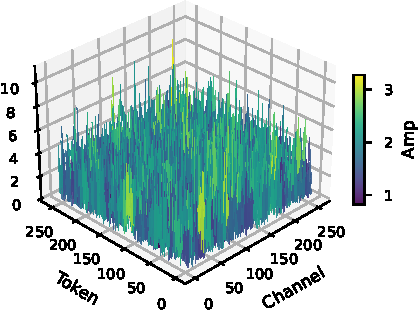
\includegraphics[width=\textwidth]{figures/visuals/comp_kv_range/comp_kv_3d_abs_dist.pdf}
    \caption{Visualization of absolute values.}
    \label{fig:comp_kv_abs_3d}
  \end{subfigure}
  \hfill % 在两图之间插入弹性间距
  % 第二张子图
  \begin{subfigure}[b]{0.43\columnwidth}
    \centering
    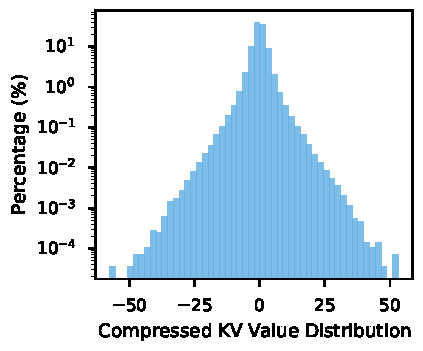
\includegraphics[width=\textwidth]{figures/visuals/comp_kv_range/comp_kv_global_dist.pdf}
    \caption{Value distribution.}
    \label{fig:comp_kv_global_dist}
  \end{subfigure}
  \caption{\textbf{Analysis of compressed KV cache values.} (a) The heatmap validates a highly uniform distribution across tokens and channels; (b) The histogram reveals concentration near 0.}
  \label{fig:comp_kv_combined}
  \vspace{-0.5em}
\end{figure}

\paragraph{Sparse-vLLM Inference Performance}
We measure decoding throughput of DeltaKV within Sparse-vLLM on a single NVIDIA RTX PRO 6000 (Blackwell), summarized in Table~\ref{tab:decode_tp}. 
Sparse-vLLM introduces minimal overhead: under full attention with 128k context, it achieves 135.0 tokens/s versus 143.2 tokens/s for native vLLM.

Enabling DeltaKV yields consistent throughput gains, especially at long contexts. At 128k, DeltaKV reaches 187.0 tokens/s, already exceeding vLLM. The advantage grows with sequence length: at 256k, DeltaKV provides a $1.7\times$ speedup, and at 512k it achieves 67.7 tokens/s versus 33.1 tokens/s for vLLM (\textbf{2}$\times$ improvement). 

Although static eviction methods (e.g., SnapKV) can achieve higher raw throughput by aggressively reducing computation, they incur significant accuracy degradation on complex tasks. DeltaKV instead offers a more favorable efficiency-accuracy trade-off.

Finally, our current implementation does not yet use a fully fused reconstruction–attention kernel. Fusing reconstruction into attention is a promising direction for further speedups. Sparse-vLLM also offers additional GPU memory savings, discussed in Appendix~\ref{app:sect:mem_eff}.

% \paragraph{开启prefill加速和省显存}

% \paragraph{RoPE}

\begin{figure*}[t]
  \centering
  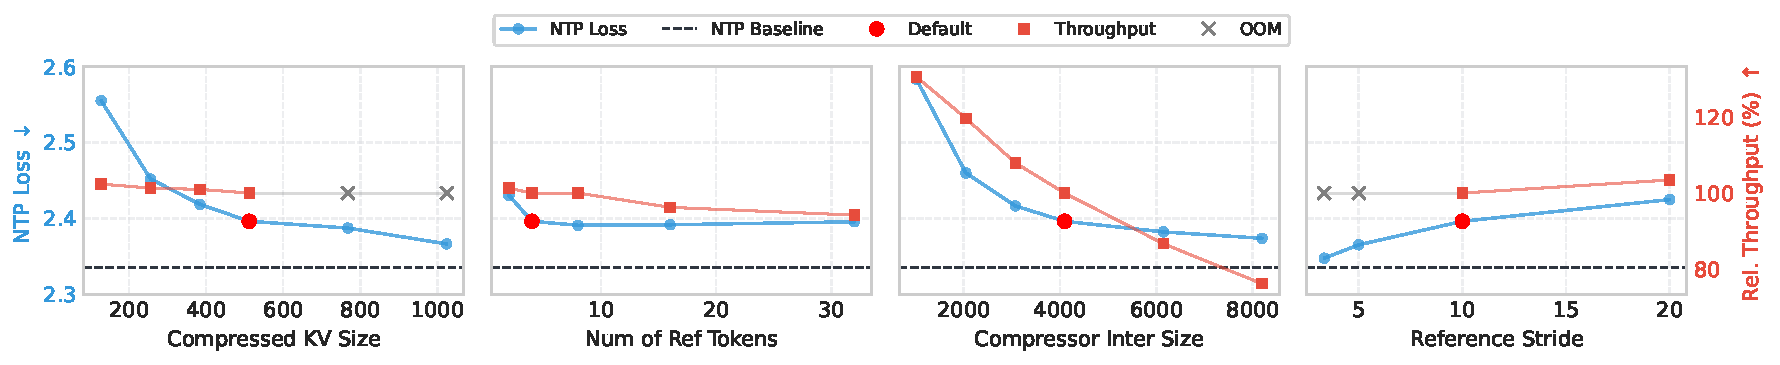
\includegraphics[width=0.99\textwidth]{figures/visuals/ablation_combined.pdf}
  \vspace{-0.5em}
  \caption{Ablation studies on model configurations.} 
  \label{fig:all_ablations}
  \vspace{-0.5em}
\end{figure*}

\begin{figure*}[hbt]
  \centering 
  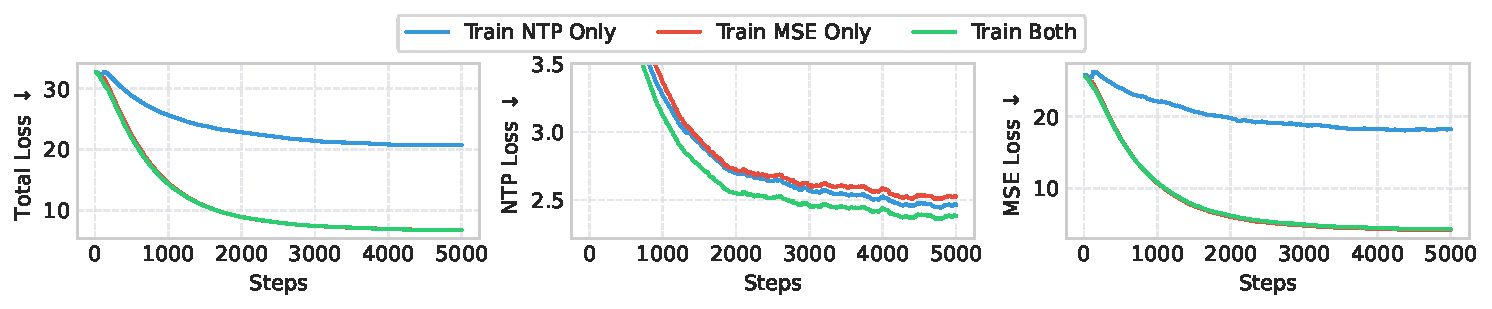
\includegraphics[width=0.99\textwidth]{figures/visuals/detach_ablation_comparison.pdf} 
  \vspace{-0.75em}
  \caption{Ablation on NTP and MSE losses.}
  \label{fig:ablation_on_ntp_mse}
  \vspace{-0.75em}
\end{figure*}

\subsection{Design Analysis and Ablations}
\label{sec:expt:analysis}

\paragraph{Compatibility with Quantization}
We analyze the value distribution of compressed KV representations produced by Qwen2.5-7B (Figure~\ref{fig:comp_kv_combined}).
%%%
The distribution is highly uniform across channels and tokens, with no prominent spikes (Figure~\ref{fig:comp_kv_abs_3d}). Most values concentrate near zero (Figure~\ref{fig:comp_kv_global_dist}), indicating strong suitability for quantization.
%%%
Applying token-wise quantization from KIVI~\cite{liu2024kivi} to $\bm{z}_\Delta$ yields near-lossless performance (Tables~\ref{tab:longbench_perf}, \ref{tab:scbench_perf}), confirming that DeltaKV's residual codes are quantization-friendly.


\paragraph{Train Short, Test Long} 
Although compressors are trained only on sequences of length 8,192, they generalize well to contexts beyond 100K tokens. 
This suggests strong length generalization. We hypothesize that this arises from performing compression before positional encoding, making the learned mapping largely position-invariant.


\paragraph{Ablation on Modules}
We conduct module ablations on Llama-3.1-8B-Inst ($2d_k=2048$). 
DeltaKV has two core components:
(1) residual construction using reference tokens, and
(2) residual compression via a lightweight module.
%%%
To ensure fair comparison, we increase $d_c$ from 512 to 768 for a $\sim$35\% KV keep ratio. Table~\ref{tab:ablation_module} shows that removing either component causes substantial degradation, confirming that both residualization and compression are essential.

\begin{table}[t]
\centering
\small
\setlength{\tabcolsep}{3pt}
\renewcommand{\arraystretch}{1.3}
\caption{Component-wise ablation study on Llama-3.1-8B.}
\label{tab:ablation_module}
\resizebox{0.99\linewidth}{!}{
\begin{tabular}{lcc ccccccc}
\toprule
\textbf{Method}  & \textbf{KR} & \textbf{CR}&
\textbf{SD} &
\textbf{MD} &
\textbf{Sum} &
\textbf{FS} &
\textbf{Syn} &
\textbf{Code} &
\textbf{Avg.} \\
\midrule
DeltaKV            & 45&30& 44.4 & 45.9 & 27.6 & 69.7 & 53.4 & 60.2 & 50.2 \\
\rowcolor[HTML]{E7F3FF} \quad w/o $f_c$ and $f_d$& 45&30& 34.4& 43.2& 24.5& 65.9& 55.1& 57.2& 46.7\\
\rowcolor[HTML]{D9EAD3} \quad w/o Ref. Tokens $\mathcal{T}$& 47&30& 39.3& 45.3& 22.1& 62.3& 50.8& 55.4& 45.9\\
\bottomrule
\end{tabular}
}
\end{table}


\paragraph{Hyperparameter Sensitivity}
We further investigate the sensitivity of DeltaKV to key hyperparameters, as illustrated in Figure~\ref{fig:all_ablations}. 
Specifically, we evaluate the throughput performance under various hyperparameters using a 128k sequence length and a batch size of 16, demonstrating the trade-off between precision and inference efficiency.
\vspace{-0.5em}
\begin{itemize}[nolistsep, left=0pt]
  \item \textbf{Compressed KV Size ($d_c$):} Increasing the dimension $d_c$ consistently yields lower NTP loss; however, excessively large dimensions lead to diminishing returns and eventually trigger Out-Of-Memory (OOM) errors. 
  
  \item \textbf{Number of Reference Tokens ($k$):} The performance gain saturates rapidly. While selecting a small number of reference tokens can lead to high average similarity, it often introduces more noise; conversely, selecting too many tokens reduces the average similarity. Thus, values of 4 or 8 serve as effective and efficient hyperparameters.

  \item \textbf{Compressor Intermediate Size ($d_h$):} While larger MLP hidden dimensions improve reconstruction quality by reducing loss, they introduce additional parameters and result in poorer inference efficiency.  

  \item \textbf{Reference Stride ($s$):} A smaller stride $s$ for reference tokens improves accuracy but linearly degrades inference throughput due to higher storage and retrieval overheads.
\end{itemize}

\vspace{-0.5em}
\paragraph{Ablation of Reconstruction and NTP Loss}
Figure~\ref{fig:ablation_on_ntp_mse} evaluates our dual-loss objective.
%%%
Since NTP loss on Fineweb-Edu~\cite{penedo2024fineweb} correlates with downstream performance, combining losses improves training effectiveness. 
%%%
Interestingly, MSE-only training reduces NTP loss, but NTP-only training does not reduce MSE. This suggests that while numerical reconstruction helps language modeling, exact KV reconstruction is not strictly required.